%%%%%%%%%%%%%%%%%%%%%%%%%%%%%%%%%%%%%%%%%%%%%%%%%%%%%%%%%%%%%%%%%%%%%%%%%%%%%%
%% Signal, Image and Video Processing (Springer Nature)
%% Manuscript: kernel surrogate modelling of PCF-SPR confinement loss
%%
%% Class options follow the SIVP submission guidelines: the journal asks for the
%% Springer Nature template with the [iicol] two-column option.  SIVP uses the
%% Springer Basic reference style with numbered citations, hence sn-basic +
%% Numbered.  Build:  pdflatex -> bibtex -> pdflatex -> pdflatex
%%
%% Figure 1 is drawn inline with TikZ (Springer asks for a single .tex source
%% and no \input).  Figures 2-4 are PDFs produced by the scripts in scripts/.
%%%%%%%%%%%%%%%%%%%%%%%%%%%%%%%%%%%%%%%%%%%%%%%%%%%%%%%%%%%%%%%%%%%%%%%%%%%%%%

\documentclass[iicol,pdflatex,sn-basic,Numbered]{sn-jnl}

\usepackage{graphicx}
\usepackage{amsmath,amssymb,amsfonts}
\usepackage{booktabs}
\usepackage{xcolor}
\usepackage{textcomp}
\usepackage{tikz}
\usetikzlibrary{calc,arrows.meta,positioning}

\definecolor{silica}{HTML}{E8E6F0}
\definecolor{analyte}{HTML}{D6EAF6}
\definecolor{goldlayer}{HTML}{EDA100}
\definecolor{pml}{HTML}{EFEFEF}
\definecolor{holeedge}{HTML}{4A3AA7}
\definecolor{figink}{HTML}{1A1A1A}
\definecolor{inkmuted}{HTML}{6B6B6B}

% Page budget: SIVP allows 10 pages. DOIs are kept in refs.bib -- scripts/
% verify_refs.py needs them, and they are the record of what was checked -- but
% suppressed in the printed list, which reclaims roughly two lines per entry.
% The .bbl declares \doi with \providecommand, so this preamble definition wins.
% To print DOIs again, delete this line and rebuild.
\newcommand{\doi}[1]{}

\raggedbottom

\begin{document}

\title[Confinement-Loss Prediction in PCF-SPR Sensors]{Confinement-loss prediction
in photonic crystal fiber SPR sensors: kernel surrogates versus generative data
augmentation}

%% The class defines \orcid{}, but it renders Orcidlogo.eps, which the official
%% template bundle does not ship -- using it breaks the build. ORCIDs are given
%% as plain text below and entered separately in Editorial Manager, which is
%% where Springer harvests them from.
\author*[1]{\fnm{Mohammad Khaleel} \sur{Hammoud}}\email{mhmdkhalil.h@gmail.com}

\author[1]{\fnm{Cem} \sur{Kalyoncu}}\email{ckalyoncu@eul.edu.tr}

\author[1]{\fnm{Ahmet} \sur{Yasli}}\email{ayasli@eul.edu.tr}

\affil*[1]{\orgdiv{Department of Computer Engineering}, \orgname{European
University of Lefke}, \orgaddress{\city{Lefke}, \country{Northern Cyprus, TR-10
Mersin, Turkey}}}

\abstract{Designing photonic crystal fiber (PCF) based surface plasmon resonance
(SPR) sensors requires repeated full-vectorial finite element simulation, which
makes iterative geometric optimisation prohibitively slow. Machine-learned
surrogates are the standard remedy, and the prevailing strategy is to grow the
scarce simulation set with a generative adversarial network before fitting a deep
network. We show that this strategy is counterproductive for the kernel models
that suit this data regime. On a 432-sample full-vectorial finite element
dataset, a Bayesian-optimised support vector regressor reaches a mean squared
error of 0.121 on the held-out geometry, against 0.314 for the published
GAN-augmented deep network, a 61\% reduction achieved without synthetic data.
Adding the same synthetic samples degrades both kernel models: the support vector
regressor rises to 0.197 and Gaussian process regression collapses entirely. We
trace the collapse to its cause, exhibiting generated sample pairs that sit 0.011
apart in scaled feature space yet differ by 0.168 in log-scaled loss, driving the
covariance matrix towards singularity. Shapley attribution identifies the outer
cladding holes as the dominant control on confinement loss, and a Monte Carlo
study identifies the lattice pitch as the dominant source of resonance
instability under fabrication error, at 98.8\% of the variance in peak
position. Timing measurements show the generative
route to be the most expensive stage of the pipeline while reducing accuracy. The
resulting surrogate is interpretable, trains in under a minute, and needs 70\%
less simulation data than comparable neural approaches.}

\keywords{Photonic crystal fiber, Surface plasmon resonance, Support vector
regression, Explainable artificial intelligence, Bayesian optimisation, Surrogate
modelling}

\maketitle

%%%%%%%%%%%%%%%%%%%%%%%%%%%%%%%%%%%%%%%%%%%%%%%%%%%%%%%%%%%%%%%%%%%%%%%%%%%%%%
\section{Introduction}\label{sec:intro}

Photonic crystal fibers coated with a thin plasmonic film form the basis of
highly sensitive surface plasmon resonance sensors for chemical and biological
detection. A guided core mode is deliberately allowed to leak towards a metal
surface; where the mode index phase-matches the surface plasmon polariton, the
confinement loss spectrum develops a sharp resonance whose wavelength tracks the
refractive index of the surrounding analyte. Locating and shaping that resonance
is a geometric design problem over the cladding lattice, the plasmonic film and
the analyte channel.

The established way to evaluate a candidate geometry is the full-vectorial finite
element method (FV-FEM), which solves Maxwell's equations on the fiber cross
section. FV-FEM is accurate but expensive, and a design study sweeping several
geometric parameters across a wavelength grid quickly becomes a multi-day
computation. This cost, rather than any modelling difficulty, is what limits
practical PCF-SPR design.

Machine-learned surrogates address the bottleneck by learning the map from
geometry and wavelength to optical response, so that a trained model replaces the
solver during the sweep. Chugh et al.~\cite{chugh2019} first applied artificial
neural networks to PCF property computation. Deep surrogates, however, need far
more training data than FV-FEM can cheaply supply, and the field's response has
been to manufacture the missing data: Zelaci et al.~\cite{zelaci2021} trained a
Wasserstein GAN with gradient penalty on their simulation set, used it to
synthesise additional samples, and reported a mean squared error (MSE) of 0.314
for the resulting augmented network.

We argue that this sequence solves a problem that need not be created. The
quantity being modelled is smooth in geometry apart from a sharp resonance peak,
the sample count is small ($N < 500$), and the input space is six-dimensional.
These are the conditions under which margin- and kernel-based regressors are
expected to outperform deep networks, and recent PCF studies are consistent with
this~\cite{kaium2024,opoku2026}. If a kernel model is accurate enough on the
original data, the augmentation step -- and the generative model behind it -- is
unnecessary.

This paper makes that case quantitatively, and then shows the augmentation step
is not only unnecessary but detrimental. The contributions are as follows.

\begin{enumerate}
\item A Bayesian-optimised support vector regression (SVR) surrogate attaining an
MSE of 0.121 on an unseen geometry from the 432 original FV-FEM samples alone: a
61\% error reduction against the published GAN-augmented deep network, and a
70\% reduction in data requirement against the closest neural
alternative~\cite{ehyaee2024}.
\item An \emph{augmentation paradox}: the same synthetic samples degrade SVR and
destroy Gaussian process regression (GPR). A mechanism is supplied rather than an
observation, exhibiting generated pairs that are geometrically near-identical yet
carry materially different targets, and showing how these drive the GPR
covariance matrix towards singularity.
\item A Shapley-value decomposition of the surrogate that attributes confinement
loss primarily to the outer cladding hole diameters, connecting the regression to
the physics of evanescent leakage rather than treating it as an opaque
predictor.
\item A Monte Carlo tolerance analysis ranking the geometric parameters by their
contribution to resonance instability under fabrication error, and a measured
comparison of the training and inference cost of every model considered.
\end{enumerate}

A preliminary version of this work appeared in the proceedings of the 34th IEEE
Signal Processing and Communications Applications Conference~\cite{hammoud2026siu}.
The present article extends it with a per-geometry cross-validation of every
model, the mechanistic account and empirical evidence for the GPR collapse, the
tolerance study of Sect.~\ref{sec:tolerance}, and an expanded treatment of the
optimisation and evaluation protocol. All figures and tables have been produced
anew for this article.

Section~\ref{sec:related} surveys related surrogate work.
Section~\ref{sec:model} describes the sensor and the FV-FEM model that generates
the data. Section~\ref{sec:method} sets out the surrogate methodology.
Section~\ref{sec:results} reports accuracy, the augmentation paradox, feature
attribution, tolerance and spectral validation. Section~\ref{sec:discussion}
discusses limitations, and Sect.~\ref{sec:conclusion} concludes.

%%%%%%%%%%%%%%%%%%%%%%%%%%%%%%%%%%%%%%%%%%%%%%%%%%%%%%%%%%%%%%%%%%%%%%%%%%%%%%
\section{Related work}\label{sec:related}

\paragraph{Neural surrogates for fiber optics.} Chugh et al.~\cite{chugh2019}
established the template: sample the geometric design space with FV-FEM, fit a
feed-forward network, and use it for fast sweeps. The approach is accurate where
data is plentiful, and its weakness is precisely that requirement. Ehyaee et
al.~\cite{ehyaee2024} pushed accuracy to an MSE of 0.084 on a PCF-SPR sensor, but
required 1,476 simulated samples to achieve it. The reported accuracy is not in
question; the associated simulation budget is the cost of obtaining it.

\paragraph{Generative augmentation.} Zelaci et al.~\cite{zelaci2021} attacked the
data requirement directly, training a WGAN-GP~\cite{gulrajani2017} on their FV-FEM
set and augmenting the training data with its output. Reported MSE improved from
0.894 to 0.314. This is the baseline against which the present work is
positioned. The improvement is measured relative to a deep network that was
itself limited by sample count, and the comparison does not establish whether a
model better suited to small datasets would have required the synthetic samples
at all.

\paragraph{Design optimisation without deep networks.} A parallel line of work
optimises PCF-SPR geometry without a deep surrogate at all. Kaziz et
al.~\cite{kaziz2024} combined a Taguchi design of experiments with machine
learning and a genetic algorithm; Romeiro et al.~\cite{romeiro2026} studied
geometric optimisation of the cladding lattice directly. Goswami et
al.~\cite{goswami2023} classified guided modes of a PCF-SPR sensor, and Fasseaux
et al.~\cite{fasseaux2024} learned refractive-index dynamics for plasmonic fiber
biosensors from measured rather than simulated spectra. These share with the
present work the premise that the sample budget, not model capacity, is the
binding constraint.

\paragraph{Kernel methods on small optical datasets.} Kalyoncu et
al.~\cite{kalyoncu2022} used $k$-nearest-neighbour regression for the loss
characteristics of bent PCF-SPR sensors. Kaium and Mollah~\cite{kaium2024} applied GPR to
PCF property estimation, and Opoku et al.~\cite{opoku2026} benchmarked ten
regressors on a simulated PCF-SPR sensor, with kernel and ensemble methods
leading. Applications of the same family of sensors continue to
broaden~\cite{shafi2026}. These results motivate our hypothesis but stop short of
testing it against a generative-augmentation baseline on identical data, which is
what we do here.

\paragraph{Interpretability.} Khatun and Islam~\cite{khatun2025} applied Shapley
additive explanations~\cite{lundberg2017} to a PCF-SPR design, isolating gold film
thickness as a driver of sensitivity, and Akter and Abdullah~\cite{akter2026}
argued for deliberately interpretable models in plasmonic sensor optimisation. We
extend that style of analysis to a multi-family cladding lattice, where the
question is not the thickness of one layer but which of several hole families
controls leakage.

%%%%%%%%%%%%%%%%%%%%%%%%%%%%%%%%%%%%%%%%%%%%%%%%%%%%%%%%%%%%%%%%%%%%%%%%%%%%%%
\section{Sensor structure and numerical model}\label{sec:model}

The dataset underlying this study was produced by FV-FEM analysis of the sensor
cross section in Fig.~\ref{fig:cross_section}, computed in COMSOL Multiphysics
with perfectly matched layers terminating the computational domain. The structure
comprises a fused-silica host, a hexagonal cladding lattice of air holes, a
plasmonic gold film, and an outer analyte channel that acts as the sensing
medium.

\begin{figure}[t]
\centering
\resizebox{\columnwidth}{!}{%
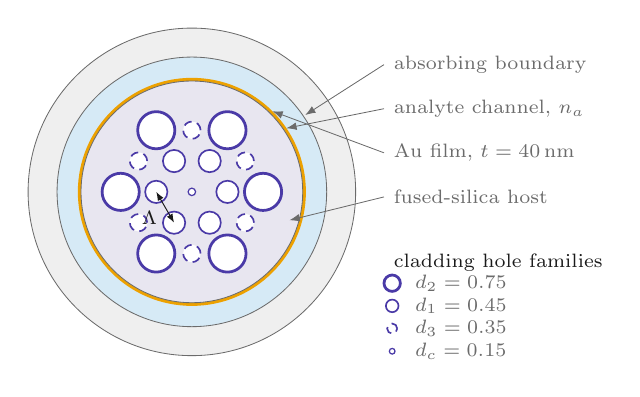
\begin{tikzpicture}[
    scale=0.80,
    every node/.style={font=\scriptsize},
    callout/.style={-{Latex[length=1.3mm]}, inkmuted, line width=0.3pt},
  ]
  \fill[pml, draw=inkmuted, line width=0.3pt] (0,0) circle (2.60);
  \fill[analyte, draw=inkmuted, line width=0.3pt] (0,0) circle (2.14);
  \fill[goldlayer] (0,0) circle (1.81);
  \fill[silica, draw=inkmuted, line width=0.3pt] (0,0) circle (1.76);

  \def\p{0.565}
  \foreach \k in {0,...,5}{
    \pgfmathsetmacro{\ang}{60*\k}
    \fill[white, draw=holeedge, line width=0.6pt]
      ({\p*cos(\ang)},{\p*sin(\ang)}) circle (0.177);
  }
  \foreach \k in {0,...,5}{
    \pgfmathsetmacro{\ang}{60*\k}
    \fill[white, draw=holeedge, line width=1.0pt]
      ({2*\p*cos(\ang)},{2*\p*sin(\ang)}) circle (0.295);
  }
  \foreach \k in {0,...,5}{
    \pgfmathsetmacro{\ang}{60*\k+30}
    \fill[white, draw=holeedge, line width=0.6pt, densely dashed]
      ({1.732*\p*cos(\ang)},{1.732*\p*sin(\ang)}) circle (0.138);
  }
  \fill[white, draw=holeedge, line width=0.45pt] (0,0) circle (0.059);

  \draw[{Latex[length=1.1mm]}-{Latex[length=1.1mm]}, figink, line width=0.35pt]
    ({\p*cos(180)},{\p*sin(180)}) -- ({\p*cos(240)},{\p*sin(240)});
  \node[figink, anchor=north east, inner sep=0.5pt]
    at ({0.5*\p*(cos(180)+cos(240))-0.10},{0.5*\p*(sin(180)+sin(240))-0.04}) {$\Lambda$};

  \draw[callout] (3.05,2.02) -- (1.80,1.22);
  \node[inkmuted, anchor=west] at (3.05,2.02) {absorbing boundary};
  \draw[callout] (3.05,1.32) -- (1.50,1.01);
  \node[inkmuted, anchor=west] at (3.05,1.32) {analyte channel, $n_a$};
  \draw[callout] (3.05,0.62) -- (1.28,1.28);
  \node[inkmuted, anchor=west] at (3.05,0.62) {Au film, $t = 40$\,nm};
  \draw[callout] (3.05,-0.08) -- (1.55,-0.45);
  \node[inkmuted, anchor=west] at (3.05,-0.08) {fused-silica host};

  \begin{scope}[shift={(3.05,-1.62)}]
    \node[figink, anchor=west] at (0,0.50) {cladding hole families};
    \fill[white, draw=holeedge, line width=1.0pt] (0.13,0.17) circle (0.13);
    \node[inkmuted, anchor=west] at (0.34,0.17) {$d_2 = 0.75$};
    \fill[white, draw=holeedge, line width=0.6pt] (0.13,-0.19) circle (0.10);
    \node[inkmuted, anchor=west] at (0.34,-0.19) {$d_1 = 0.45$};
    \fill[white, draw=holeedge, line width=0.6pt, densely dashed]
      (0.13,-0.55) circle (0.08);
    \node[inkmuted, anchor=west] at (0.34,-0.55) {$d_3 = 0.35$};
    \fill[white, draw=holeedge, line width=0.45pt] (0.13,-0.91) circle (0.045);
    \node[inkmuted, anchor=west] at (0.34,-0.91) {$d_c = 0.15$};
  \end{scope}
\end{tikzpicture}}
\caption{Cross section of the modelled PCF-SPR sensor. Three families of air
holes sit on a hexagonal lattice of pitch $\Lambda$ in a fused-silica host, with
a central defect hole of diameter $d_c$. Light leaking from the core couples to
the surface plasmon supported by the gold film. Legend diameters are in
\textmu m and give the nominal design; the dataset sweeps them over the ranges
in Table~\ref{tab:design}.}\label{fig:cross_section}
\end{figure}

Nineteen air holes in three diameter families form the cladding, together with a
small central defect hole. The gold film is 40\,nm thick, with permittivity taken
from the Johnson and Christy measurements~\cite{johnson1972}. The refractive index
of the silica host follows the Sellmeier relation~\cite{rifat2017}

\begin{equation}
n^2(\lambda) = 1 + \sum_{i=1}^{3} \frac{B_i\lambda^2}{\lambda^2 - C_i},
\label{eq:sellmeier}
\end{equation}

with $B_i$, $C_i$ the standard Sellmeier coefficients for fused silica. The
predicted quantity is the confinement loss, obtained from the imaginary part of
the effective index as~\cite{zelaci2021}

\begin{equation}
L_c = \frac{40\pi}{\ln(10)\,\lambda}\,\mathrm{Im}(n_\mathrm{eff})\times 10^{4}
\quad [\mathrm{dB/cm}].
\label{eq:confinement_loss}
\end{equation}

$L_c$ peaks at the phase-matching condition, so the resonance region, where the
function is least smooth, is what a surrogate must reproduce.

%%%%%%%%%%%%%%%%%%%%%%%%%%%%%%%%%%%%%%%%%%%%%%%%%%%%%%%%%%%%%%%%%%%%%%%%%%%%%%
\section{Surrogate modelling methodology}\label{sec:method}

\subsection{Dataset and preprocessing}\label{sec:dataset}

We use the FV-FEM dataset of Zelaci et al.~\cite{zelaci2021}, so that the
comparison against their GAN-augmented network is made on identical data. It
contains 432 labelled samples over six input variables: analyte refractive index
$n_a$, wavelength $\lambda$, lattice pitch $\Lambda$, and the three cladding hole
diameters $d_1$, $d_2$, $d_3$. Table~\ref{tab:design} summarises the sampled
design space.

\begin{table}[t]
\caption{Sampled design space. Nine geometric configurations, each evaluated for
three analytes over a 16-point wavelength grid, give $9 \times 3 \times 16 = 432$
FV-FEM samples.}\label{tab:design}
\begin{tabular*}{\columnwidth}{@{\extracolsep\fill}lll}
\toprule
Variable & Role & Sampled values \\
\midrule
$n_a$      & analyte index   & 1.33, 1.34, 1.35 \\
$\lambda$  & wavelength      & 16-point grid \\
$\Lambda$  & lattice pitch   & 0.15, 0.20, 0.24 \\
$d_1$      & inner holes     & 0.25, 0.45 \\
$d_2$      & outer holes     & 0.55, 0.75 \\
$d_3$      & interstitial holes & 0.15, 0.35 \\
$d_c$      & central defect  & 0.15 (fixed) \\
\midrule
$L_c$      & target          & $10^{-3}$--$59.1$\,dB/cm \\
\botrule
\end{tabular*}
\footnotetext{Geometric values are the dataset's own column values. The
$\lambda$ column is in units of 100 nm, so the 16-point grid spans
500--800\,nm; the Sellmeier index of fused silica over that span,
$n = 1.462$--$1.453$, matches the dataset's $\mathrm{Re}(n_\mathrm{eff})$ of
1.42--1.46.}
\end{table}

The target spans nearly five orders of magnitude and is dominated by the
resonance peak, so we regress the log-scaled response
$y = \log_{10}(L_c \times 10^{8})$. This both compresses the dynamic range and
makes squared error a sensible loss across the whole spectrum rather than one
concentrated at the peak. Inputs are min-max scaled to $[0,1]$, which matters for
the radial basis function (RBF) kernel because an unscaled wavelength axis would
otherwise dominate the distance metric.

\subsection{Evaluation protocol}\label{sec:protocol}

Random train-test splitting is inappropriate for this dataset. The 432 samples
are not independent: they derive from nine geometric configurations, each
contributing a full wavelength sweep. A random split places samples from the
same geometry on both sides of the partition, so that the model interpolates
within a spectrum it has already observed. The resulting error understates the
quantity of interest, which is generalisation to a geometry that has not been
simulated.

We therefore evaluate at the level of geometries, under two protocols:

\begin{itemize}
\item \textbf{Fixed partition.} The 7--1--1 split of~\cite{zelaci2021}:
configurations 1--7 for training, 8 for validation, 9 held out for test. This
reproduces the published protocol exactly and is the basis for the headline
comparison.
\item \textbf{Leave-one-geometry-out (LOGO).} Each of the nine configurations
serves in turn as the test set, the other eight as training data. This gives
nine independent estimates and, unlike the fixed partition, reports the variance
across geometries as well as the mean.
\end{itemize}

The fixed partition constitutes a single draw and may favour a model that happens
to suit configuration 9. LOGO is the more informative of the two protocols; both
are reported.

\subsection{Support vector regression}\label{sec:svr}

SVR fits a function deviating from the observed targets by at most $\epsilon$
while remaining as flat as possible, penalising only the samples falling outside
that tube~\cite{smola2004}. Writing $C$ for the box constraint and $\xi_i$,
$\xi_i^{*}$ for the slack variables, the primal problem minimises
$\tfrac{1}{2}\|w\|^{2} + C\sum_{i}(\xi_i + \xi_i^{*})$ subject to the two
$\epsilon$-tube constraints; the full formulation, its dual and the
Karush-Kuhn-Tucker conditions are given in Online Resource 1, Sect.~S1. The
kernel is radial basis,
$K(x_i,x_j) = \exp(-\gamma\|x_i - x_j\|^{2})$.

The relevant property is that the fit is determined by the support vectors, the
samples on or outside the tube boundary, rather than by all 432 points equally.
Near the resonance, where the response turns sharply, this concentrates model
capacity where the function is least smooth, which accounts for the method's
tolerance of a small sample count.

\subsection{Gaussian process regression}\label{sec:gpr}

GPR places a Gaussian process prior $f(x)\sim\mathcal{GP}(m(x),k(x,x'))$ over
functions, so that the posterior mean and covariance at a test input $x_*$
are~\cite{rasmussen2006}

\begin{align}
\bar{f}_* &= K_*^{\top}\left[K + \sigma_n^{2}I\right]^{-1}y,
\label{eq:gpr_mean}\\
\mathrm{cov}(f_*) &= K_{**} - K_*^{\top}\left[K + \sigma_n^{2}I\right]^{-1}K_*,
\label{eq:gpr_cov}
\end{align}

with $K$ the training covariance, $K_*$ the train-test covariance and
$\sigma_n^{2}$ the noise variance. We use an RBF kernel with an additive white
noise term, which regularises the inversion in \eqref{eq:gpr_mean} and
\eqref{eq:gpr_cov}. GPR offers calibrated uncertainty, which SVR does not, and
that makes its behaviour under augmentation in Sect.~\ref{sec:paradox}
diagnostic: the same smoothness assumption that yields the uncertainty estimate
is what the synthetic data violates.

\subsection{Hyperparameter optimisation}\label{sec:bayesopt}

$C$, $\gamma$ and $\epsilon$ interact, and grid search over three coupled
continuous parameters wastes most of its budget in uninformative regions. We
instead use Gaussian-process Bayesian optimisation~\cite{snoek2012} with expected
improvement, 32 evaluations, and log-uniform priors over
$C\in[1,2000]$, $\gamma\in[10^{-4},1]$ and $\epsilon\in[10^{-4},10^{-1}]$,
scoring each candidate by three-fold cross-validated MSE on the training
partition only. The selected configuration and the full search space are
tabulated in Online Resource 1, Sect.~S2.

%%%%%%%%%%%%%%%%%%%%%%%%%%%%%%%%%%%%%%%%%%%%%%%%%%%%%%%%%%%%%%%%%%%%%%%%%%%%%%
\section{Results}\label{sec:results}

\subsection{Predictive accuracy}\label{sec:accuracy}

Table~\ref{tab:benchmark} reports every model under both protocols. On the fixed
partition the optimised SVR reaches an MSE of 0.121, against 0.314 for the
GAN-augmented deep network of~\cite{zelaci2021} and 0.894 for the unaugmented
network -- a 61\% error reduction relative to the augmented baseline, obtained
without generating a single synthetic sample. GPR reaches 0.185, also well ahead
of both neural baselines.

\begin{table*}[t]
\caption{Accuracy of each surrogate under both evaluation protocols. Rows are
metrics and columns are models, so that the fixed-partition result and the
distribution over the nine leave-one-geometry-out folds can be read against each
other for a given model. Lower is better throughout; dashes mark figures not
reported in the source work.}\label{tab:benchmark}
\small
\begin{tabular*}{\textwidth}{@{\extracolsep\fill}lccccc}
\toprule
& \multicolumn{2}{c}{Published neural baselines} & \multicolumn{2}{c}{This work} & \\
\cmidrule{2-3}\cmidrule{4-5}
Metric & Deep net~\cite{zelaci2021} & GAN-augmented~\cite{zelaci2021}
& \textbf{SVR} & GPR & ML-enhanced ANN~\cite{ehyaee2024} \\
\midrule
Fixed-partition MSE       & 0.894 & 0.314 & \textbf{0.121} & 0.185 & 0.084 \\
LOGO mean MSE             & ---   & 0.825 & \textbf{0.246} & ---   & ---   \\
LOGO standard deviation   & ---   & 0.609 & \textbf{0.226} & ---   & ---   \\
Training samples          & 432   & 432 + synth. & \textbf{432} & 432 & 1{,}476 \\
Synthetic data            & no    & yes   & \textbf{no}    & no    & no    \\
\botrule
\end{tabular*}
\footnotetext{MSE is computed on the $\log_{10}$-scaled confinement loss defined
in Sect.~\ref{sec:dataset}.}
\end{table*}

The LOGO protocol matters more, and it separates the models further. Averaged
over the nine held-out geometries the SVR attains an MSE of 0.246 with a standard
deviation of 0.226, against 0.825 $\pm$ 0.609 for the augmented benchmark. The
gap in the standard deviation is the more useful number for a design tool: a
surrogate that is accurate on average but occasionally wrong by a wide margin on
an unfamiliar geometry cannot be trusted to drive an optimisation loop. Per-fold
results are given in Online Resource 1, Sect.~S3.

The comparison with Ehyaee et al.~\cite{ehyaee2024} requires careful statement.
Their ML-enhanced ANN attains an MSE of 0.084, lower than the 0.121 reported
here, but does so using 1,476 training samples against 432. Since each training
sample is an FV-FEM solution, this difference dominates the cost of the entire
pipeline, and a 70\% reduction in that cost for a 0.037 increase in MSE
constitutes a favourable trade-off in a design context.

The mechanism underlying this result is the one anticipated in
Sect.~\ref{sec:svr}. A deep network fits a global function and requires
sufficient samples to constrain it throughout the input domain, a condition nine
geometries do not meet. SVR instead concentrates representational capacity on the
support vectors bounding the transition between the high- and low-loss regions,
and extrapolates from that boundary rather than from a globally interpolated
surface.

\subsection{The augmentation paradox}\label{sec:paradox}

The augmentation strategy of~\cite{zelaci2021} was next applied to the kernel
models, generating synthetic samples with the same WGAN-GP configuration and
adding them to the training partition. Since synthetic data is known to benefit
models limited by sample count, the question addressed here is whether it also
benefits models that are not so limited.

Table~\ref{tab:augmentation} shows the support vector regressor degrading from
0.121 to 0.197 and Gaussian process regression failing outright, and the
direction of change is consistent across the leave-one-geometry-out folds
(Online Resource 1, Sect.~S3). Augmentation is therefore not introducing noise
that averages out over folds; it is displacing the fit. On this evidence,
WGAN-GP augmentation does not improve predictive accuracy in either case.

\begin{table}[t]
\caption{Effect of adding GAN-generated samples to the training partition, split
out here from the accuracy comparison because it measures a different thing:
not which model is best, but what augmentation does to a model that did not need
it.}\label{tab:augmentation}
\begin{tabular*}{\columnwidth}{@{\extracolsep\fill}lccc}
\toprule
Model & Real only & Augmented & Change \\
\midrule
SVR & 0.121 & 0.197 & $+63\%$ \\
GPR & 0.185 & 23.844 & collapse \\
GPR (LOGO) & --- & 52.86 & collapse \\
\midrule
Deep network~\cite{zelaci2021} & 0.894 & 0.314 & $-65\%$ \\
\botrule
\end{tabular*}
\footnotetext{Fixed-partition MSE except where marked. The GPR
leave-one-geometry-out mean is carried from~\cite{hammoud2026siu}; the
generator is retrained per fold, so fold-level values scatter widely
(32.7--76.1 in a partial re-run) and the mean is the stable quantity. The
neural row is reproduced from~\cite{zelaci2021} for contrast: the same
synthetic samples that help a data-starved network harm both kernel models.}
\end{table}

The GPR failure is the informative case, because it is not a gradual degradation
but a numerical breakdown, and its cause is identifiable. A GAN is a
probabilistic sampler with no constraint tying it to Maxwell's equations, so
nothing prevents it from emitting two samples that are geometrically almost
identical while carrying materially different losses. Such a pair is physically
impossible -- the same geometry at the same wavelength has one confinement loss --
but it is entirely consistent with a generator that has learned the marginal
distributions without the physics.

To confirm this we generated 50,000 samples, found each one's nearest neighbour
in the scaled feature space, and ranked the resulting pairs by the ratio of
target discrepancy to feature distance. Table~\ref{tab:gan_fail} lists the three
worst. The leading pair sits 0.011 apart in a space scaled to the unit cube, yet
its targets differ by 0.168 in log-scaled loss, a 45\% discrepancy in physical
units. The search protocol is detailed in Online Resource 1, Sect.~S4.

\begin{table}[t]
\caption{The three most contradictory nearest-neighbour pairs among 50,000
GAN-generated samples, ranked by target discrepancy per unit of feature
distance. Quantities run down the rows and pairs across the columns; each column
is one pair of generated samples that are near-identical in the input space but
carry incompatible targets.}\label{tab:gan_fail}
\small
\begin{tabular*}{\columnwidth}{@{\extracolsep\fill}lccc}
\toprule
Quantity & Pair A & Pair B & Pair C \\
\midrule
Feature distance         & 0.0111 & 0.0089 & 0.0088 \\
Target 1 ($\log_{10}$)   & 4.4466 & 4.3722 & 4.3280 \\
Target 2 ($\log_{10}$)   & 4.6144 & 4.4958 & 4.4347 \\
Target discrepancy       & 0.1678 & 0.1236 & 0.1067 \\
Discrepancy/distance     & 15.09  & 13.81  & 12.06 \\
\botrule
\end{tabular*}
\footnotetext{Feature distance is Euclidean in the min-max scaled
seven-dimensional space the generator was trained on; targets are the
$\log_{10}$-scaled confinement loss.}
\end{table}

For GPR the consequence is numerical failure rather than degradation. The
posterior in
\eqref{eq:gpr_mean} requires inverting $[K + \sigma_n^{2}I]$. Two inputs at
distance 0.011 produce near-identical rows in $K$, so the matrix approaches
singularity; the white-noise term $\sigma_n^{2}$ is what normally absorbs this,
but it is calibrated to the noise level of the real data and is far too small to
absorb a 0.168 jump. The inverse is then dominated by the ill-conditioned
directions and the predictive variance explodes. SVR survives because its
$\epsilon$-insensitive loss simply admits both contradictory points as bounded
support vectors: the fitted function is degraded, but the optimisation remains
well posed.

Generative augmentation therefore exchanges a data-quantity limitation for a
data-consistency one. For a model whose accuracy is limited by sample count this
exchange may be favourable; for a model that is not so limited it is
unambiguously detrimental.

This is a physical instance of a failure the wider machine-learning literature has
begun to document. Shumailov et al.~\cite{shumailov2024} showed that training on
model-generated data drives progressive degradation, and Juwara et
al.~\cite{juwara2024} found synthetic augmentation beneficial only under
conditions that must be checked rather than assumed. Our setting differs from the
recursive loop those studies analyse, in that augmentation is performed once from
a generator trained on real data. A single generation affords no opportunity for
error to compound, so the degradation observed here must have another source.
That source is the absence of a physical constraint: the generator is free to
violate the single-valuedness that the underlying Maxwell problem guarantees.

\subsection{What the surrogate learned}\label{sec:xai}

A surrogate that is accurate but opaque is of limited use in design, where the
question is not only what the loss will be but which parameter to change. We
applied Shapley additive explanations~\cite{lundberg2017} to the trained SVR,
which decomposes each prediction into additive per-feature contributions.

Figure~\ref{fig:shap} gives the resulting global ranking. The outer cladding
diameters $d_2$ and $d_3$ dominate, together accounting for 63\% of total
attribution, followed by the lattice pitch $\Lambda$ at 23\%. Wavelength
contributes 9\%, and the innermost holes $d_1$ barely register at 2\%.

\begin{figure}[t]
\centering
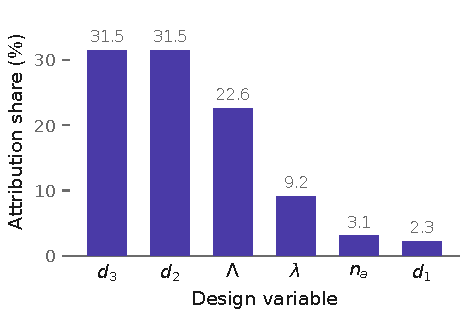
\includegraphics[width=\columnwidth]{figs/fig2_shap_importance.pdf}
\caption{Global Shapley attribution for the trained SVR, expressed as each
variable's share of total attributed magnitude. The outer cladding families
$d_2$ and $d_3$ jointly account for 63\% of the attribution; the innermost holes
$d_1$ are nearly inert.}\label{fig:shap}
\end{figure}

This ordering is physically consistent, and reading it against the geometry of
Fig.~\ref{fig:cross_section} explains why. Confinement loss is set by how much of
the core field reaches the gold surface, and the outer hole families are what
that field must traverse to get there. Enlarging $d_2$ or $d_3$ raises the index
contrast of the outer cladding, tightening confinement and suppressing leakage.
The innermost holes sit inside the field maximum, where they shape the mode
profile but do very little to gate its escape -- hence their negligible
attribution. That the model recovers this ordering from data alone, without being
told the physics, is evidence it has learned the leakage mechanism rather than a
correlation.

\subsection{Manufacturing tolerance}\label{sec:tolerance}

Fiber drawing does not reproduce a design exactly, so a surrogate is useful for
design only if it can also identify which deviations matter. The geometric
inputs were perturbed with Gaussian noise at 1\%, 3\% and 5\% relative standard
deviation, 100 Monte Carlo trials were run at each level, and the induced
scatter in the predicted resonance wavelength was recorded. The experiment was
then repeated perturbing one variable at a time in order to attribute that
scatter. Peak jitter grows from 2.3\,nm at 1\% tolerance to 10.1\,nm at 5\%;
the complete tables are given in Online Resource 1, Sect.~S6.

The pitch $\Lambda$ dominates, contributing 5.49\,nm of jitter and 98.8\% of
the variance in peak position, while the three hole diameters together
contribute under 0.7\,nm. This establishes a fabrication priority: pitch
uniformity along the drawn fiber governs whether a device matches its
calibration, whereas tolerance on the cladding holes may be relaxed without
appreciable spectral cost.

Two points qualify these values. First, they supersede the corresponding figures
in~\cite{hammoud2026siu}, which were computed at a baseline geometry lying
outside the sampled design space of Table~\ref{tab:design}; the surrogate was
there extrapolating, and the resulting peak search returned grid endpoints in
roughly half of all trials. The values above are obtained at a sampled geometry
with a boundary-guarded peak search, under which no trial is rejected at any
tolerance level. Second, the analysis perturbs the surrogate inputs only, and
therefore propagates geometric tolerance but not the predictive error of the
surrogate itself.

% ---------------------------------------------------------------------------
% UNITS -- RESOLVED.  The `lambda' column of data.xlsx is in units of 100 nm,
% confirmed by the authors and independently by the Sellmeier index of fused
% silica: over 500-800 nm it gives n = 1.462-1.453, matching the dataset's
% Re(n_eff) of 1.42-1.46, whereas 5-8 um gives 1.34-0.64 and 5-8 nm gives ~1.0.
%
% The SIU paper printed "27.63 nm/RIU".  The number 27.63 is correct as a peak
% shift in nm per 0.01 RIU step; the unit label was wrong.  The sensitivity is
% 2763 nm/RIU, which this article reports.
% ---------------------------------------------------------------------------

\subsection{Computational cost}\label{sec:timing}

The argument for a surrogate rests on cost, so the cost was measured rather than
asserted. Every model was timed on the same machine (AMD Ryzen 5 5500U, 12
threads, CPU only), the same 432-sample dataset and the same software stack.
Figure~\ref{fig:timing} reports the result.

\begin{figure}[t]
\centering
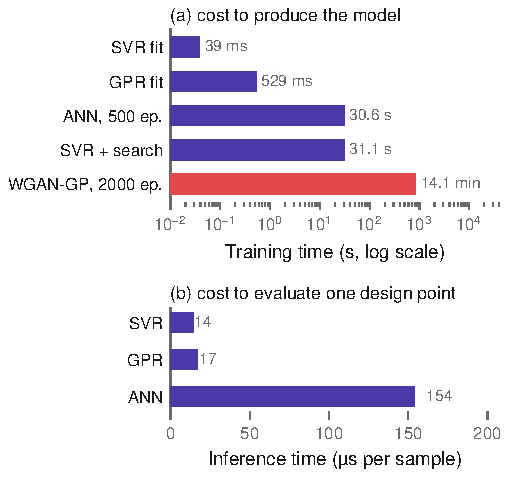
\includegraphics[width=\columnwidth]{figs/fig5_timing.pdf}
\caption{Measured cost of each model, on identical hardware and data.
Panel~(a) gives the time to produce a usable model, on a logarithmic scale
spanning four orders of magnitude; WGAN-GP training (highlighted) is the
dominant term. Panel~(b) gives the per-sample inference cost, the quantity that
governs a design sweep. Absolute values are hardware-specific; the ratios are
not.}\label{fig:timing}
\end{figure}

Three observations follow. First, fitting the SVR at fixed hyperparameters takes
39\,ms, and the full 32-evaluation Bayesian search 31.1\,s, so the entire
surrogate is produced in well under a minute. Second, inference costs
14\,\textmu s per design point against 154\,\textmu s for the ANN, an order of
magnitude that matters when a sweep evaluates $10^{5}$ candidate geometries.
Third, and most relevant to Sect.~\ref{sec:paradox}, training the WGAN-GP
generator alone takes 847\,s, some four orders of magnitude more than the SVR
fit it is intended to support. The augmentation route therefore incurs by far
the largest computational cost in the pipeline while, on this dataset, reducing
accuracy. These figures exclude the FV-FEM solutions themselves, which dominate
the total budget in every case and are common to all models.

\subsection{Spectral validation}\label{sec:spectral}

Aggregate error statistics can conceal a surrogate that is accurate on average
yet incorrect in spectral shape. Sweeping the trained SVR across the full
wavelength range at fixed geometry reproduces the expected behaviour: a single
well-formed resonance shifting monotonically to longer wavelengths as the
analyte index rises from 1.33 to 1.35, in near-uniform steps of 27.93 and
27.33\,nm, giving a spectral sensitivity of 2763\,nm/RIU. The phase-matching condition was never supplied to
the model, so recovery of both the direction and the regularity of this shift
indicates that the underlying coupling has been captured rather than the
training spectra memorised. The predicted spectra are shown in the Online
Supplement, Sect.~S7.


%%%%%%%%%%%%%%%%%%%%%%%%%%%%%%%%%%%%%%%%%%%%%%%%%%%%%%%%%%%%%%%%%%%%%%%%%%%%%%
\section{Discussion and limitations}\label{sec:discussion}

The results support a claim narrower than a general superiority of kernel methods
over deep learning. Deep surrogates underperform here not by virtue of their
depth, but because nine geometries do not adequately constrain a global function
approximator; synthesising further data addresses the symptom rather than the
cause. Where sufficient real simulation data is available the neural result
of~\cite{ehyaee2024} is stronger; the regime addressed here is the more common
one in which it is not.

Three limitations bound this work. First, the analysis rests entirely on FV-FEM
output, so the surrogate inherits any error present in the numerical model, and
experimental validation on a drawn fiber remains necessary. Fabrication effects
outside the model, including gold surface roughness, material impurity and
ellipticity of the drawn holes, will affect sensitivity and signal-to-noise
ratio in ways that surrogate accuracy cannot anticipate.

Second, the surrogate is interpolative within the sampled design space of
Table~\ref{tab:design}, and is not a substitute for FV-FEM outside those ranges.
The LOGO protocol measures generalisation to an unseen geometry within the
sampled envelope rather than beyond it.

Third, the augmentation paradox is demonstrated for a single generator
architecture on a single dataset. The mechanism identified here, namely a
generator subject to no physical constraint emitting inconsistent near-duplicate
pairs, is not specific to WGAN-GP, and is expected to affect any unconstrained
generative augmentation supplying a kernel model. Establishing this requires
evaluation of generators constrained to respect the governing equations, which
would provide the additional data volume without the accompanying inconsistency.
A consistency check on generated samples, of the kind performed in
Sect.~\ref{sec:paradox}, should in any case precede the use of synthetic data in
this setting~\cite{juwara2024}.

%%%%%%%%%%%%%%%%%%%%%%%%%%%%%%%%%%%%%%%%%%%%%%%%%%%%%%%%%%%%%%%%%%%%%%%%%%%%%%
\section{Conclusion}\label{sec:conclusion}

We have shown that a Bayesian-optimised support vector regressor predicts PCF-SPR
confinement loss more accurately than a GAN-augmented deep network on identical
data -- a 61\% error reduction -- using only the 432 original FV-FEM samples and
no synthetic data. Under leave-one-geometry-out validation the advantage holds in
both mean and variance.

The augmentation step that the surrogate literature has converged on is, for this
class of model, actively harmful. Adding GAN-generated samples raises SVR error by
63\% and collapses GPR entirely, and we have traced the collapse to generated
sample pairs that are geometrically near-identical yet carry incompatible
targets, driving the covariance matrix towards singularity. Generative
augmentation exchanges a shortage of data for an inconsistency in it; that
exchange is only worth making for a model that cannot function without the
volume.

Beyond accuracy, the surrogate yields design guidance: Shapley attribution
identifies the outer cladding diameters as the dominant control on confinement
loss, and Monte Carlo tolerance analysis identifies the lattice pitch as the
dominant source of resonance instability. Together these indicate both the
parameter to tune and the parameter to hold, at a training cost of tens of
milliseconds and an evaluation cost of tens of microseconds.

%%%%%%%%%%%%%%%%%%%%%%%%%%%%%%%%%%%%%%%%%%%%%%%%%%%%%%%%%%%%%%%%%%%%%%%%%%%%%%
\backmatter

\bmhead{Supplementary information}

Online Resource 1 contains the SVR dual formulation and KKT conditions
(Sect.~S1), the Bayesian optimisation search space and selected hyperparameters
(Sect.~S2), per-fold leave-one-geometry-out results (Sect.~S3), the WGAN-GP
configuration and contradiction-search protocol (Sect.~S4), a GPR kernel and
regulariser ablation (Sect.~S5), and the full Monte Carlo tolerance tables
(Sect.~S6).

\bmhead{Acknowledgements}

The authors thank the Department of Computer Engineering, European University of
Lefke, for computational support.

\section*{Declarations}

\textbf{ORCID.} M.K. Hammoud 0009-0004-4262-867X; C. Kalyoncu
0000-0002-2027-0695; A. Yasli 0000-0003-4654-3222.

\textbf{Funding.} This work was supported by the Research Fund of the European
University of Lefke, project number BAPKO.0392620.

\textbf{Conflict of interest.} The authors declare no competing interests.

\textbf{Data availability.} The dataset analysed in this study was generated in
the course of~\cite{zelaci2021} and is publicly available at
\url{https://github.com/Aimen-Zelaci/SPRPCF\_ANN}.

\textbf{Ethics approval and consent to participate, consent for publication, and
materials availability.} Not applicable.

\textbf{Code availability.} Available from the corresponding author on reasonable
request.

\textbf{Author contribution.} M.K.H. implemented the surrogate models, the
augmentation experiments and the analyses, and drafted the manuscript. C.K.
supervised the machine-learning methodology. A.Y. provided the photonic
modelling and FV-FEM dataset. All authors revised and approved the manuscript.

\textbf{Prior publication.} A preliminary version was presented at the 34th IEEE
Signal Processing and Communications Applications Conference
(SIU~2026)~\cite{hammoud2026siu}; Sect.~\ref{sec:intro} describes how this
article extends it. All figures and tables are newly prepared.

\bibliography{refs}

\end{document}
